\section{Filtro 2: Merge}

\subsection{Explicacion}
El filtro de merge consiste en tomar 2 imagenes del mismo tamaño y un float value (Con valor entre 0 y 1) y promediar los pixeles de cada imagen para crear una tercer imagen usando como parametro value. \\

\subsection{Implementacion 1}
La primera implementacion pide trabajar con floats procesando la mayor cantidad de pixeles posibles por iteracion. \\

Como sabemos que la cantidad de pixeles de las imagenes es un multiplo de 4 vamos a trabajar de a 4 pixeles que nos permite operar sin tener que procuparnos por salirnos de la memoria alocada a la imagen. \\

Para procesar los pixeles del merge vamos a usar 2 registros XMM para guardar los 4 pixeles como bytes que obtenemos de la memoria y 2 registros mas para guardar copias de los mismos. Ademas como vamos a utilizar una funcion auxiliar vamos a usar 4 registros XMM mas para guardar los resultados de la funcion. Y por ultimo tenemos los dos valores guardados en float en los registros XMM15 (value) y XMM14 (1 - value). \\

\begin{figure}[h!]
	\centering
	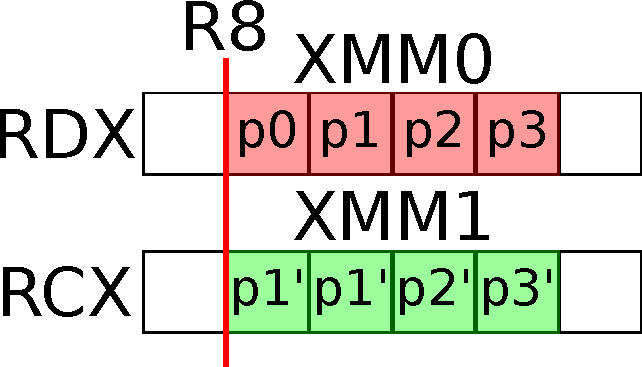
\includegraphics[scale=0.5]{images/MergeASM1_0}
\end{figure}

Ademas vamos a usar los siguientes registros de proposito general: \\
RDX puntero a la primera imagen \\
RCD puntero a la segunda imagen \\
R9 iterador en y
R8 iterador en x (En bytes)

Es importante aclarar que antes de entrar en la iteracion creamos los registros XMM14 y XMM15 moviendo el value (XMM0) a XMM15 sufleandolo a todo el registro para que me quede v ; v ; v ; v y luego moviendo a XMM14 4 floats (1.0 ; 1.0 ; 1.0 ; 1.0) que tenemos almacenado en memoria y luego restandole a XMM14 XMM15.

Antes de comenzar a iterar en y inicializo el iterador de y en 0. \\

Al principio de cada ciclo de x inicializo el iterador en x en 0. \\

Luego muevo a los registros XMM0 y XMM1 los datos de la primera y segunda imagen. Ademas hago una copia de cada uno en XMM2 y XMM3 (XMM2 = XMM0, XMM3 = XMM1). \\

Ahora procedo a llamar a addPixels 4 veces y a guardar los valores en los registros XMM4, XMM5, XMM6, XMM7. \\

addPixels es una funcion auxiliar que hace lo siguiente: \\

Mueve los valores de las copias a XMM0 y XMM1 (XMM0 = XMM2, XMM1 = XMM3). Luego los desenpaqueta de byte a word y de word a doubleword usando el registro XMM10 el cual posee todos ceros. Los convierte a float, luego multiplica a XMM0 por XMM15 y a XMM1 por XMM14. \\

Luego de hacer esto queda en XMM0 a * v ; r * v ; g * v ; b * v y en XMM1 a * (1 - v) ; r * (1 - v) ; g * (1 - v) ; b * (1 - v). \\

Suma ambos y los pasa de float a doubleword, de doubleword a word y de word a byte. \\

Al final shiftea las copias (XMM2 y XMM3) 4 bytes a la derecha para que quede el siguiente pixel a procesar en los primeros 4 bytes de los mismos. \\

Una vez que tengo los valores lo unico que me falta hacer es pasarlo a memoria, incremento el iterador de x (R8 += 16) y hacer la comparacion, si no llegue al final de la fila de pixeles itero nuevamente. \\

Una vez que termine con la fila aumento el puntero de RDX en una fila, y hago lo mismo con el de RCX. Incremento en uno el iterador de y (R9++) y me fijo si llegue al final de la imagen, en caso de no ser asi itero nuevamente en y. \\

\subsection{Implementacion 2}
La segunda implementacion pide trabajar con enteros procesando la mayor cantidad de enteros posibles por iteracion.

Al igual que en la primera implementacion vamos a trabajar de a 4 pixeles al mismo tiempo por que nos permite iterar de manera segura.

Al igual que en la primera implementacion vamos a usar los registros XMM14 y XMM15 para guardar los valores por los cuales vamos a multiplicar los pixeles. Para calcularlos vamos a mover value (XMM0) a XMM15, luego lo shufleamos para que los 4 floats que entran en XMM15 sean v, movemos a XMM14 los floats en memoria (8192.0 ; 8192.0 ; 8192.0 ; 8192.0) y multiplicamos XMM15 por XMM14. Para finalizar le restamos a XMM14 XMM15 y convertimos ambos registros de float a doubleword. Al terminar esto nos queda: \\
	XMM15 = v * 8192 ; v * 8192 ; v * 8192 ; v * 8192
	XMM14 = 8192 - v * 8192 ; 8192 - v * 8192 ; 8192 - v * 8192 ; 8192 - v * 8192 = 8192 * (1 - v) ; 8192 * (1 - v) ; 8192 * (1 - v) ; 8192 * (1 - v) \\
Se elijio 8192 que es $2^{13}$ por que es el numero mas chico posible para usar y que el error que tenga al procesar la imagen este dentro de los parametros de los test.

Ademas vamos a usar los registros XMM0 a XMM7 para tomar los valores de memoria y desenpaquetar. Y XMM10 que es un registro con ceros tambien para desenpaquetar.

\begin{figure}[h!]
	\centering
	\includegraphics[scale=0.5]{images/MergeASM2_0}
\end{figure}

Los registros de proposito general que vamos a usar son los mismos que en la primera implementacion.

Antes de comenzar a iterar en incializamos el iterador de y (R9) en 0.

Al principio de cada iteracion de x inicializo el iterador de x (R8) en 0.

Luego muevo a XMM0 y XMM4 los grupos de pixeles de la primera y segunda imagen. Luego desenpaqueto de byte a word y de word a doubleword para que me queden los siguientes registros:
	XMM0 = p0
	XMM1 = p1
	XMM2 = p2
	XMM3 = p3
	XMM4 = p0'
	XMM5 = p1'
	XMM6 = p2'
	XMM7 = p3'

Despues multiplico XMM0, XMM1, XMM2 y XMM3 por XMM15 y lo shifteo 13 bits a la derecha, esto me da (p * 8192v) / 8192 = p * v

Hago lo mismo con XMM4, XMM5, XMM6 y XMM7 pero esta vez multiplicando por XMM14 y me quedan (p * 8192(1 - v)) / 8192 = p * (1 - v)

Luego me quedan en los registros cada pixel multiplicado por v o (1 - v) segun corresponda. Con un poco de paciencia y ingenio podemos enpaquetar las cosas para que queden los 4 pixeles como byte en un solo registro como se muestra en la siguiente imagen. Lo mismo funciona tanto para los dos grupos de pixeles.

\begin{figure}[h!]
	\centering
	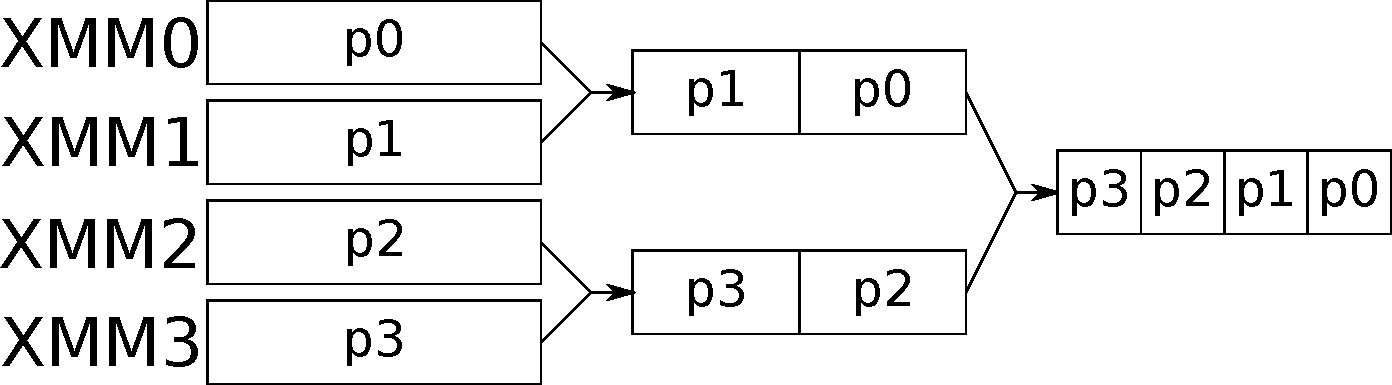
\includegraphics[scale=0.5]{images/MergeASM2_1}
\end{figure}

Al final nos queda en XMM0 p3 * v ; p2 * v ; p1 * v ; p0 * v y en XMM4 p3' * (1 - v) ; p2' * (1 - v) ; p1' * (1 - v) ; p0' * (1 - v)

Para terminar solo necesito sumarlos y moverlos a memoria. Esto se puede hacer con un solo mov.

Luego al igual que en la primera implementacion checkeo si llegue al final sino itero en x nuevamenete y hago lo mismo con y.

\subsection{Resultados}
Para la experimentacion vamos a correr las 3 implementaciones (La version de C compilada con optimizaciones de nivel 3) con la imagen de lena brindada por la catedra (multiplos de 16x16, hasta 320x320), se corren 100 veces cada tamaño y despues se saca un promedio y se grafica el maximo, el minimo y el promedio.

\begin{figure}[h!]
	\centering
	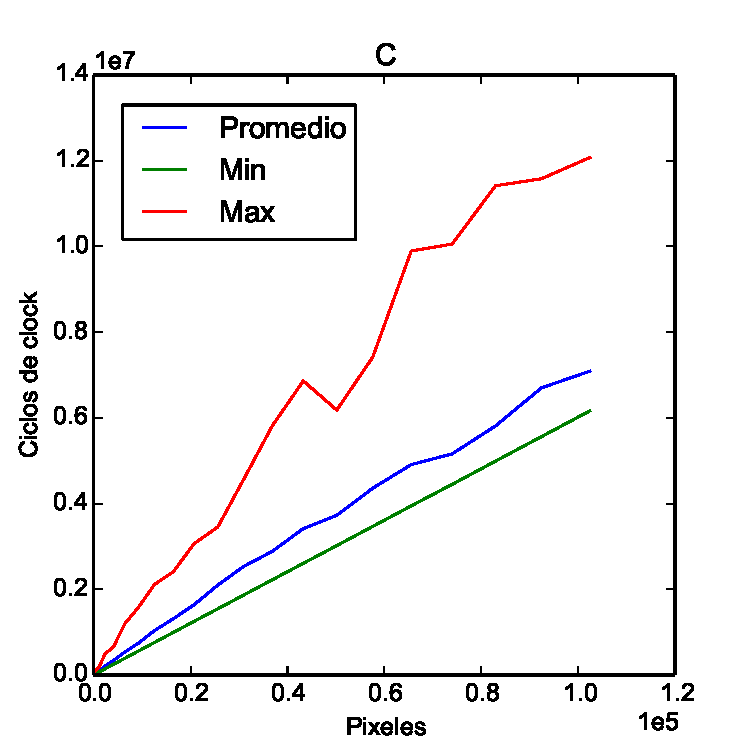
\includegraphics[scale=0.45]{images/c_merge}
	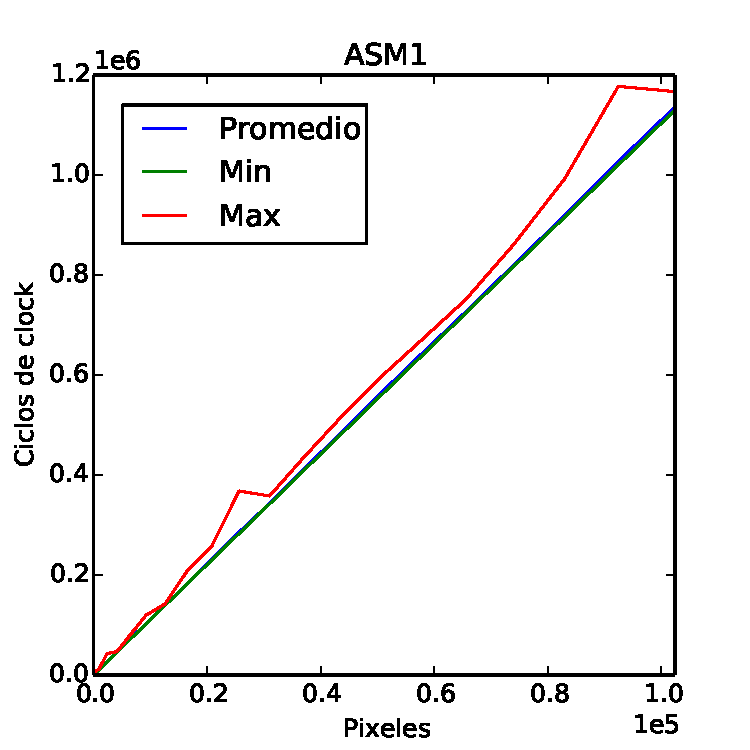
\includegraphics[scale=0.45]{images/asm1_merge}
	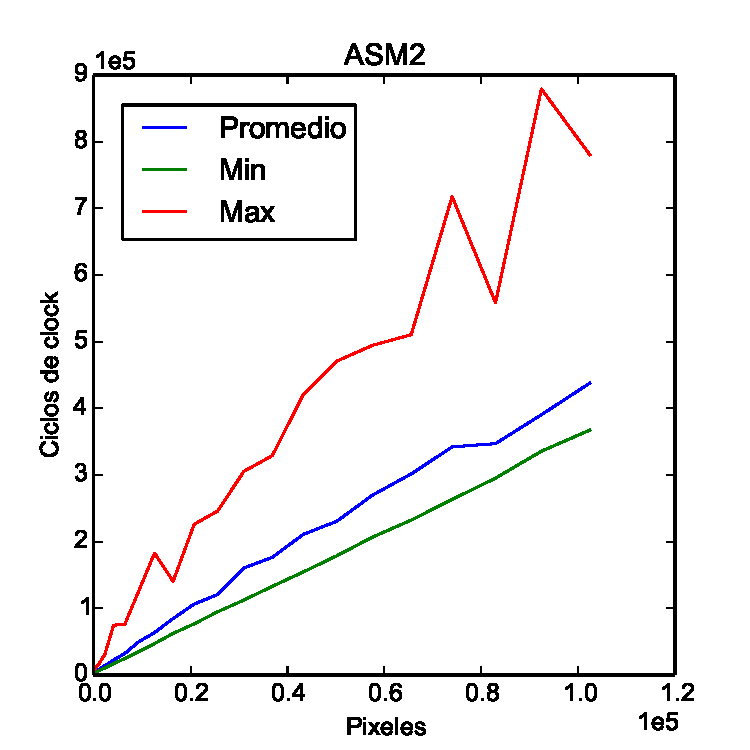
\includegraphics[scale=0.45]{images/asm2_merge}
\end{figure}

Tambien graficamos los 3 promedios en un grafico para ver cual de ellos es el mas rapido en general. Y para ver mejor la diferencia entre ASM1 y ASM2 los graficamos aparte.

\begin{figure}[h!]
	\centering
	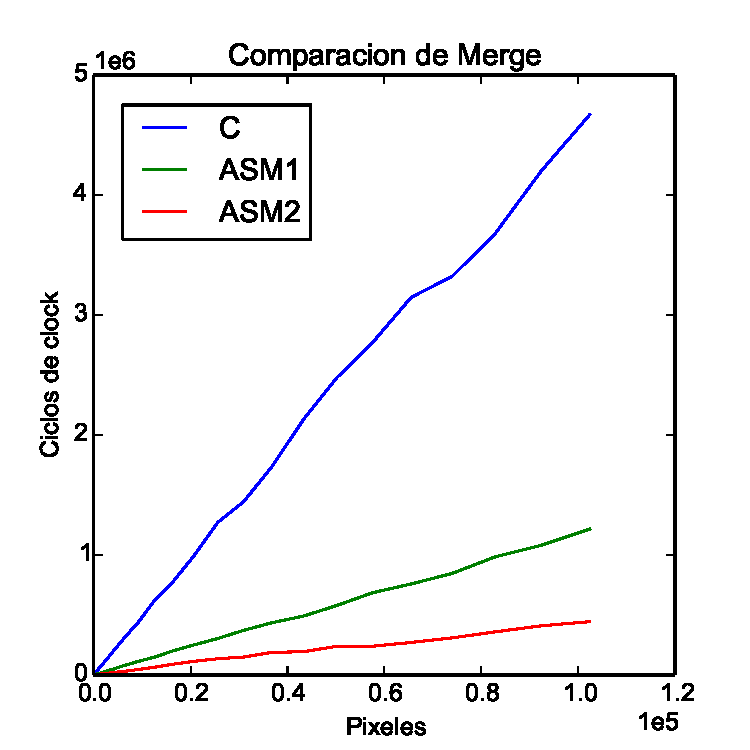
\includegraphics[scale=0.5]{images/c_asm1_asm2_merge_comp}
	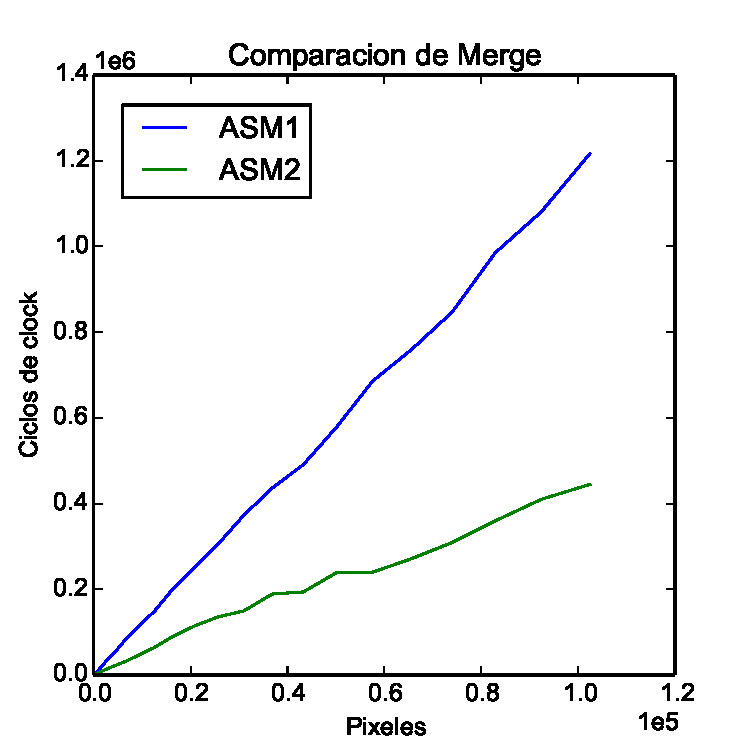
\includegraphics[scale=0.5]{images/asm1_asm2_merge_comp}
\end{figure}

Tambien queremos ver que la imagen no modifique el tiempo de ejecucion, tanto el codigo de C com el de ASM no poseen ningun salto condicional que depende de el valor de los pixeles.

\begin{figure}[h!]
	\centering
	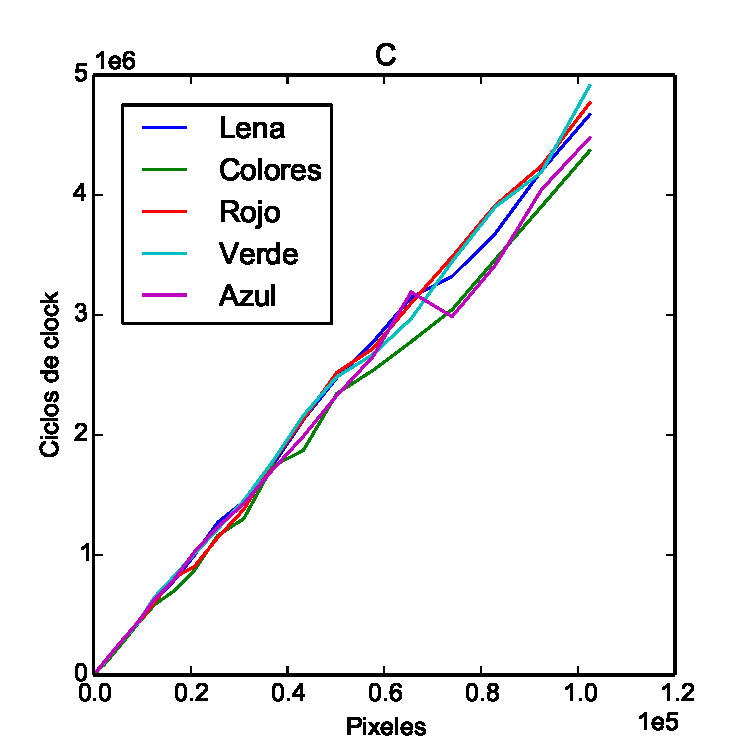
\includegraphics[scale=0.45]{images/c_merge_lena_colors}
	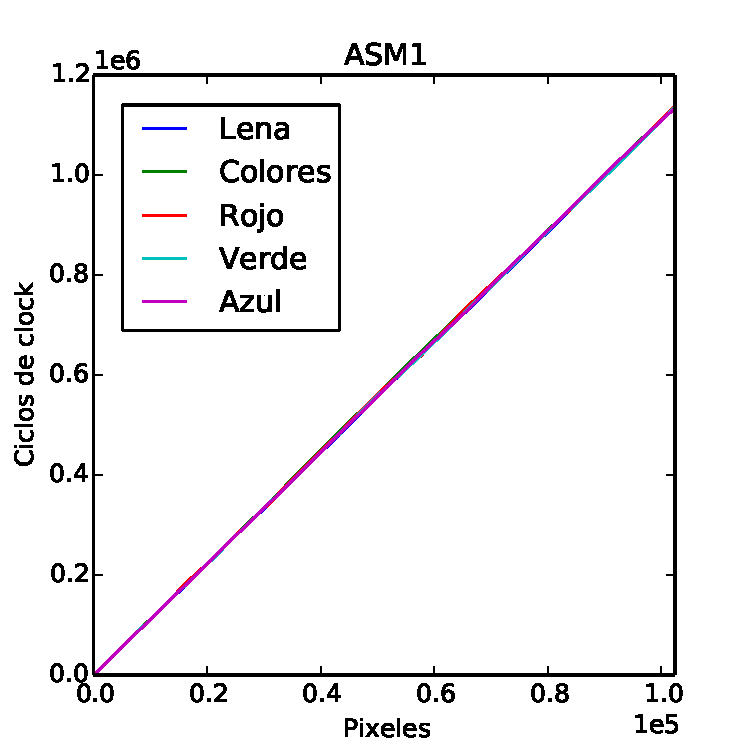
\includegraphics[scale=0.45]{images/asm1_merge_lena_colors}
	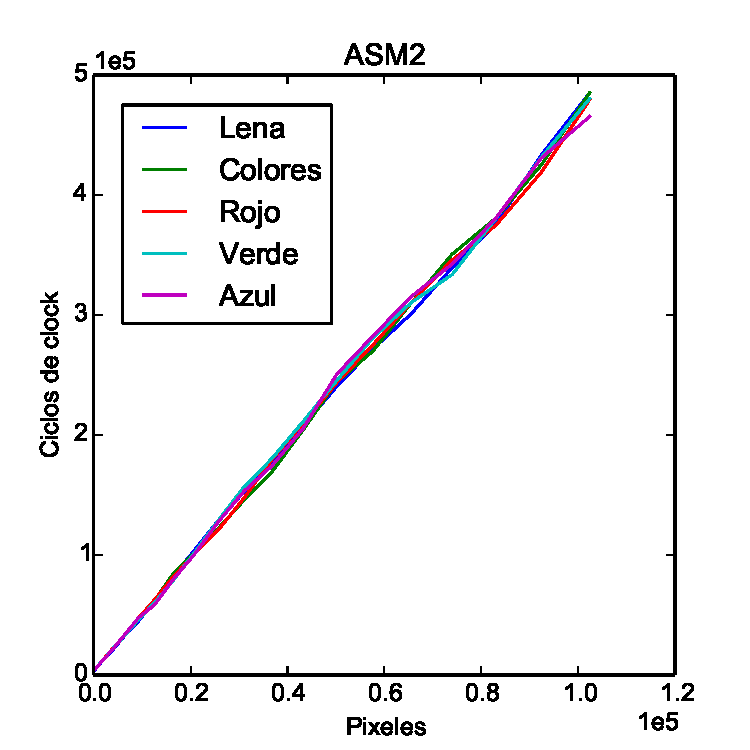
\includegraphics[scale=0.45]{images/asm2_merge_lena_colors}
\end{figure}

\subsection{Conclusion}